\documentclass[A4paper,10pt]{paper}
\usepackage{xeCJK}
\usepackage{listings}
\usepackage{hyperref}
\usepackage{amsmath,amssymb,amsthm}
\usepackage{xcolor}

%\lstset
%{
%    basicstyle=\ttfamily,
%    numbers=left,
%    % numberstyle=\tiny,
%    keywordstyle=\color[RGB]{0, 0, 255},
%    commentstyle=\color[RGB]{0, 128, 0},
%    frame=shadowbox,
%    rulesepcolor=\color{red!20!green!20!blue!20},
%    showspaces=false,
%    showstringspaces=false,
%    extendedchars=false,
%    showtabs=false,
%    tabsize=4, breaklines,
%    xleftmargin=2em,xrightmargin=2em, aboveskip=1em
%  }

\lstset{numbers=none,
  numberstyle=\scriptsize,
  flexiblecolumns=false,
  language=Haskell,
  frame=shadowbox,
  basicstyle=\ttfamily\small,
  breaklines=true,
  extendedchars=true,
  escapechar=\%,
  texcl=true,
  showstringspaces=false,
  keywordstyle=\bfseries,
  tabsize=4}
  
\setCJKmainfont{AR PL UKai CN}

\title{FOPL-Homework 5}
\author{昂伟 PB11011058}
\date{ \today }

\begin{document}

\maketitle

\section*{Problem 1}
	\begin{lstlisting}
	Bool Halt(P, n); // true if P halts
	                 // false if P does not halt
	void K(P)		 
	{ 
		if (Halt(P, P) == false) 
			return true;
		else {
			while(1) { }
		}
	}
	\end{lstlisting}
	\paragraph{分析} 若K(K) = true, 则Halt(K, K) = false, 即K(K) = false,矛盾.
	
\section*{Problem 2}
	\subsection*{(a)}
	\paragraph{} 1个类被加入,即productExp类;没有类被修改.
	
	\subsection*{(b)}
	\paragraph{} 没有类被加入,n + 1 个类被修改.
	
	\subsection*{(c)}
	\paragraph{} m个类被修改,1个类被加入.
	
	\subsection*{(d)}
	\paragraph{} 1个类被加入, 没有类被修改.
	
	\subsection*{(e)}
	\paragraph{} 只增加新的表达式类型而不增加新的表达式操作时,才用标准做法只须增加一个新的表达式类而不会修改其他类.
	
	\subsection*{(f)}
	\paragraph{} 只增加表达式操作而不增加新的表达式类型时,采用visitor设计模式可以只增加一个表达式操作类而不修改其他类.
	
\section*{Problem 3}
	\subsection*{(a)}
	\paragraph{} 
	\begin{minipage}{.45\textwidth}
		\centering
%		\begin{table}[!htbp]	
		\textit{Activation Records}	
		\begin{tabular}{l|l|c}
		\hline
		(0) 		& r			 	& (1) 	\\ 	\cline{2-3}
	     		& cp				& (3)   \\  	\cline{2-3}
		\hline
		(1)	Point(...)	& access link 	& (0) 	\\	\cline{2-3}
	   			& x				& 2.1 	\\	\cline{2-3}
	   			& y 				& 4.2 	\\	\cline{2-3}
	   			& equals			& .		\\	\cline{2-3}
	   			& distance 		& . 		\\	\cline{2-3}
		\hline
		(2) Point part of cp & access link & (0) \\ \cline{2-3}
				& x				& 3.6	\\	\cline{2-3}
				& y 				& 4.9  	\\	\cline{2-3}
				& equals 		& .		\\	\cline{2-3}
				& distance 		& .		\\	\cline{2-3}
		\hline
		(3) 	ColorPt(...) & access link 	& (2)		\\ 	\cline{2-3}
	 			& c  			& red	\\	\cline{2-3}
	 			& equals 		& .		\\
	 	\hline 
	 	(4) 	cp.distance(r) &	access link & (2)	\\	\cline{2-3}
	 			& q				& (r)	\\	\cline{2-3}
	 	\hline
	 	
		\end{tabular}
%		\end{table}
	\end{minipage}
	\makeatletter\
	\begin{minipage}{.3\textwidth}
		\centering
		\textit{Closures}\\
		<(1), $\bullet$> \\
		<(1), $\bullet$> \\
		<(2), $\bullet$> \\
		<(2), $\bullet$> \\
		<(3), $\bullet$> \\
		\end{minipage}
		\makeatletter\
		\begin{minipage}{.2\textwidth}
		\centering
		\textit{Compiled Codes}\\
		$\textbar\ code\ for\ equals \textbar $\\
		$\textbar\ code\ for\ distance \textbar$ \\
		$\textbar\ code\ for\ cpt\ equals \textbar $
	\end{minipage}
	\subsection*{(b)}
	\paragraph{} 首先在活动记录(4)中搜索x,发现没有定义x,接着沿着access link(2)找到活动记录(2),然后在活动记录(2)中搜索x,发现x = 3.6
	
	\subsection*{(c)} 
	\paragraph{} 首先在cp指向的活动记录(3)中搜索x,发现没有x,接着沿着活动记录(3)的access link(2)找到活动记录(2),然后在活动记录(2)中搜索x,发现x
	
	\subsection*{(d)}
	\paragraph{} distance函数定义在Point类中,且没在子类ColorPt中重新定义,并且只用到基类中的数据成员x,y.
	
	\subsection*{(e)}
	\paragraph{} 不会放在栈上,而是放在堆上. 因为只有当程序不再使用对象时才能释放对象占用的活动记录,放在栈上可能导致提前释放活动记录,导致引用对象出错.

\section*{Problem 4}
	\subsection*{(a)}
	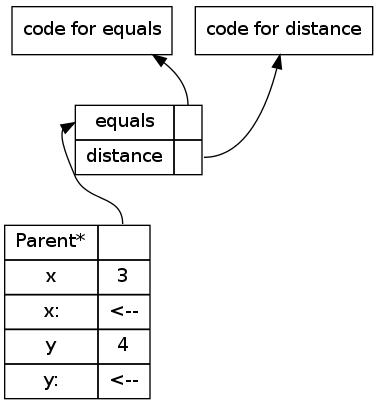
\includegraphics[width=0.5\textwidth]{./pro4a.png}
	\subsection*{(b)}
	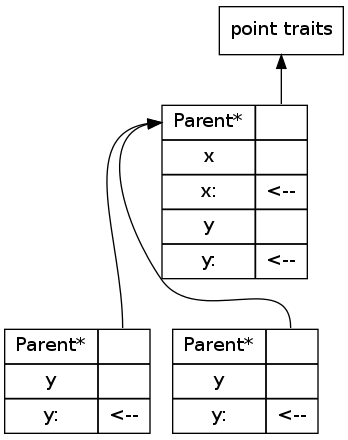
\includegraphics[width=0.5\textwidth]{./pro4b.png}
	\subsection*{(c)}
	\paragraph{} 只复制被复制对象的fields,并将被创建对象的父指针指向被复制对象.
	
	\subsection*{(d)}
	\paragraph{} 有可能导致改变父节点的对象的子对象的行为发生改变,即当该对象的子对象引用该对象的父对象的方法时发生问题.
	
\subsection*{Problem 5}
	\subsection*{(a)}
	\paragraph{} 不需要,因为可以将子类的vtable组织成和父类vtable同构的结构.
	
	\subsection*{(b)}
	\paragraph{} 2n个entries,其中n个entries用来存放offset(虽然单继承时都为0).第一种方案实现的编译器对单继承和多继承对象的处理没有不同,都需要额外的n个entries来保存offset.
	
	\subsection*{(c)}
	\paragraph{} 采用第一种方案实现的多继承编译器在调用虚函数前先将\emph{this}指针加上对应虚函数entry中的offset,传给该函数作为参数,除此之外没有其他额外开销.
	
	\subsection*{(d)}
	\paragraph{} 采用第二种方案实现的编译器只需维护n个enries用于存储虚函数地址.该方案下,调用虚函数时可能会发生一次额外的函数调用和一次无条件跳转(\emph{goto}).编译器会为使用多继承的函数生成额外的\emph{chunk}.
	
	\subsection*{(e)}
	\paragraph{} 采用第一种方案的编译器不可以链接运行. 第二种方案可以.
	
\section*{Problem 6}
	\subsection*{(a)}
%	\begin{figure}[!htbp]
	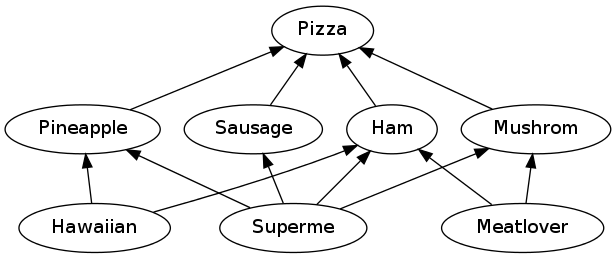
\includegraphics[width=0.8\textwidth]{./pro6.png}
%	\end{figure}		

	\subsection*{(b)}
	\paragraph{} 命名冲突.
	
	\subsection*{(c)}
	\paragraph{} Interface: Pizza, Sausage, Ham, Pineapple, Mushroom.
	\paragraph{} Class: Supreme, Hawaiian, Meatlover.
	
	\subsection*{(d)}
	\paragraph{} C++多继承时无需查表,程序运行效率. Java接口实现简单,直观.
	
\end{document}
